\begin{center}
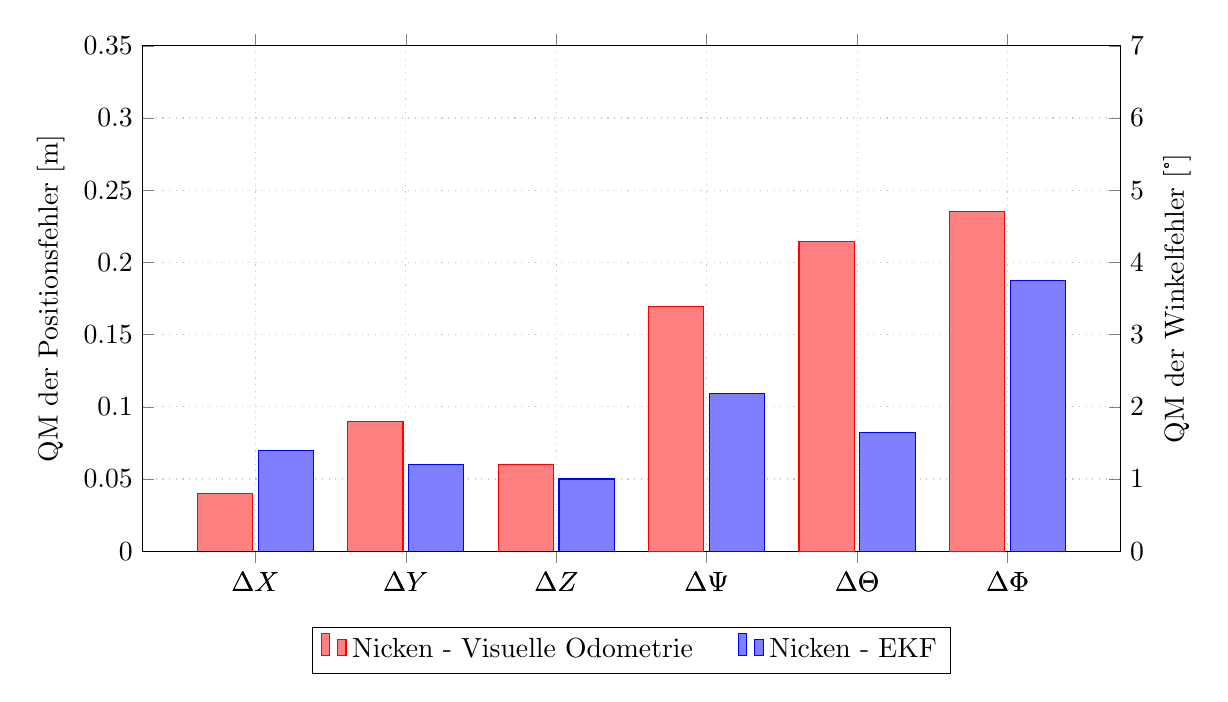
\begin{tikzpicture}
\begin{axis}[
	ybar,
	ymax=0.35,
	ymin=0,
	bar width=20pt,
	scaled y ticks = false,
	y tick label style={/pgf/number format/fixed},
%	enlarge y limits={0.4,upper},
	enlarge x limits=0.15,
	legend style={at={(0.5,-0.15)},
	legend style={/tikz/every even column/.append style={column sep=0.5cm}},
	anchor=north,legend columns=-1},
	ylabel={QM der Positionsfehler \lbrack m\rbrack},
%	symbolic x coords={\Delta,y,z},
	xtick={1,2,3,4,5,6},
	xticklabels={$\Delta X$, $\Delta Y$, $\Delta Z$, $\Delta \Psi$, $\Delta \Theta$, $\Delta \Phi$},
%	xtick=data,
%	every node near coord/.style={/pgf/number format/fixed,/pgf/number format/use comma, anchor=west},
%	nodes near coords,
%	nodes near coords align={vertical},
	width=14cm,
	height=8cm,
	grid=major,
    	grid style={dotted,lightgray!80!white},
    	scaled y ticks = false,
]
\addplot[
%	every node near coord/.append style={xshift=-0.9cm},
%	nodes near coords=\raisebox{0.7cm}{\pgfmathprintnumber\pgfplotspointmeta},
	color=red,
	fill=red!50!white,
	bar shift=-11pt,
] coordinates {(1,0.04) (2,0.09) (3,0.06)};
\addplot[
%	every node near coord/.append style={xshift=-0.12cm},
%	nodes near coords=\raisebox{0.7cm}{\pgfmathprintnumber\pgfplotspointmeta},
	color=blue,
	fill=blue!50!white,
	bar shift=11pt,	
] coordinates {(1,0.07) (2,0.06) (3,0.05)};
\addplot[fill opacity=0.0,draw=none,] coordinates {(4,0) (5,0) (6,0)};	%dummy
\legend{Nicken - Visuelle Odometrie,Nicken - EKF}
\end{axis}

\begin{axis}[
%	scale only axis,
	ybar,
	ymax=7,
	ymin=0,
	bar width=20pt,
%	enlarge y limits={0.4,upper},
	enlarge x limits=0.15,
	legend style={at={(0.5,-0.15)},
	anchor=north,legend columns=-1},
	axis y line*=right,
	ylabel={QM der Winkelfehler \lbrack °\rbrack},
%	symbolic x coords={\Delta,y,z},
	xtick={1,2,3,4,5,6},
	xticklabels={$\Delta X$, $\Delta Y$, $\Delta Z$, $\Delta \Psi$, $\Delta \Theta$, $\Delta \Phi$},
%	xtick=data,
%	bar shift=0pt,
%	every node near coord/.style={/pgf/number format/fixed,/pgf/number format/use comma, anchor=west},
%	nodes near coords,
%	nodes near coords align={vertical},
	width=14cm,
	height=8cm,
    	scaled y ticks = false,
]
\addplot[fill opacity=0.0,draw=none,] coordinates {(1,0) (2,0) (3,0)};	%dummy
\addplot[
%	every node near coord/.append style={xshift=-0.9cm},
%	nodes near coords=\raisebox{0.7cm}{\pgfmathprintnumber\pgfplotspointmeta},
	color=red,
	fill=red!50!white,
	bar shift=-11pt,	
] coordinates {(4,3.39) (5,4.29) (6,4.70)};
\addplot[
%	every node near coord/.append style={xshift=-0.12cm},
%	nodes near coords=\raisebox{0.7cm}{\pgfmathprintnumber\pgfplotspointmeta},
	color=blue,
	fill=blue!50!white,
	bar shift=11pt,	
] coordinates {(4,2.18) (5,1.64) (6,3.75)};
\end{axis}
\end{tikzpicture}
\end{center}